\section{Theoretical Framework}
\subsection{Breast Cancer}
\qquad Breast Cancer is a malignant tumor, a collection of cancer cells, arising from the cells of the breast. Breast cancer typically originates in the cells of the lobules, milk-producing glands, or the ducts, the passages that drain milk from the lobules to the nipple \cite{breastCancer}. \\

	There are several types of breast cancer, but the type of breast cancer is classified by the specific cells in the breast that are afflicted by the disease. The most common types are ductal carcinoma in situ, invasive ductal carcinoma, and invasive lobular carcinoma.The terms "in situ" and "invasive" refer to the extent of the spread of the cancer. "In situ," also called as "non-invasive," means that the cancer has not spread, while "invasive," also called as "infiltrating," means that the cancer has spread to the surrounding breast tissue \cite{breastCancerTypes}.

\begin{enumerate}
	\item \textit{Ductal carcinoma in situ} \\
	Ductal carcinoma in situ (DCIS) is the most common type of non-invasive breast cancer \cite{breastCancerOrgDCIS}. DCIS is described by cancer cells that line the milk ducts of the breast. Since it is non-invasive, it is contained only in the milk ducts, but immediate treatment is still necessary, for it may eventually become invasive \cite{ACSDCIS}.

	\item \textit{Invasive ductal carcinoma} \\
	Invasive ductal carcinoma (IDC) is the most common type of breast cancer accounting for about 80\% of all breast cancers. IDC means that the cancer has spread to the surrounding breast tissue originating from the milk ducts. Over time, the cancer may spread to the lymph nodes and other parts of the body \cite{breastCancerOrgIDC}.

	\item \textit{Invasive lobular carcinoma} \\
	Invasive lobular carcinoma (ILC) is the second most common type of breast cancer after IDC. ILC is characterized by cancer that originated from the lobules. Like IDC, the cancer cells have the potential to spread to the lymph nodes and other areas of the body \cite{breastCancerOrgILC}.
	
\end{enumerate}

	As mentioned, the most common symptom of breast cancer is a new lump or mass. A painless, hard mass with irregular edges is evidently cancer, but, in other breast cancer cases, the mass can be tender, soft, rounded, and painful. Other possible symptoms include:

\begin{itemize}
	\item swelling of all or part of a breast even if no distinct lump is felt
	\item skin irritation or dimpling
	\item breast or nipple pain
	\item nipple retraction
	\item redness, scaliness, or thickening of the nipple or breast skin
	\item nipple discharge
\end{itemize}

	In invasive breast cancer, there are cases where, after spreading to the lymph nodes under the arm or around the collar bone, swelling may occur there, even before the original tumor in the breast becomes large enough to be felt \cite{ACSSymptoms}. \\

	The survival rates for breast cancer depends solely on the stage or the extent of the cancer. Generally, the survival rates are higher for women with earlier stage cancers. According to the National Cancer Institute's SEER database from people diagnosed with breast cancer from 2007 to 2013, the 5-year relative survival rate for women with stage 0 or stage I breast cancer is close to 100\%; the 5-year relative survival rate for women with stage II breast cancer is approximately 93\%; the 5-year survival rate for stage III breast cancers is about 72\%; Lastly, the 5-year relative survival rate for women with stage IV breast cancers is about 22\%. Fortunately, there are many widely available treatment options even for this stage of cancer \cite{cancerPrognosis}. \\

	Treatment depends on the biology and behavior of breast cancer. Treatment options and recommendations are very personalized and depend on several factors \cite{cancerTreatmentSpecific}:

\begin{itemize}
	\item the stage of the tumor
	\item the patient's age, general health, menopausal status, and preferences
	\item the presence of known mutations in inherited breast cancer genes
\end{itemize}

	Cancer care teams comprising of several health care professionals such as surgeons, radiologists, oncologists, physycian assistants, oncology nurses, social workers, pharmacists, counselors, nutritionists, and others work together to create a patient's overall treatment plan which is a summary of planned cancer treatment. Some of the most common treatment options include \cite{cancerTreatmentSpecific}:

\begin{enumerate}
	\item Surgery \\
	Surgery is the removal of the tumor and some surrounding healthy tissue for good measure. There are two type of surgery namely lumpectomy and mastectomy. Lumpectomy is the removal of the tumor and a small, cancer-free area of healthy tissue around the tumor. Often, there could be several follow-up treatments after surgery such as radiation therapy. On the other hand, mastectomy is the surgical removal of the entire breast.

	\item Radiation therapy \\
	Radiation therapy is the use of high-energy x-rays of other particles to destroy cancer cells. Some types include external-beam radiation therapy, intra-operative radiation therapy, and brachytherapy. External-beam radiation therapy is radiation given to the affected area from a machine outside the body. Intra-operative radiation therapy is given using a probe in the operating room. Lastly, brachytherapy is done by placing radioactive sources into the tumor. \\

	Radiation therapy is usually given over a set period of time indicated by the regimen given by the radiation oncologist. However, this kind of treatment may cause side effects such as fatigue, swelling of the breast, redness and/or skin discoloration, and pain/burning in the skin where the radiation was directed.

	\item Chemotherapy \\
	Chemotherapy is the use of drugs to destroy cancer cells usually by inhibiting the cancer cells' ability to grow and spread. The common ways by which chemotherapy drugs are applied include an intravenous tube placed into a vein using a needle, an injection under the skin or into a muscle, or a pill or capsule that is swallowed. Chemotherapy may also be given before surgery to shrink larger tumors to make surgery easier, and after surgery to minimize the risk of recurrence. Common drugs prescribed include capecitabine, carboplatin, cisplatin, cyclophosphamide, docetaxel, doxorubicin, pegylated liposomal doxorubicin, epirubicin, fluorouracil, gemcitabine, methotrexate, paclitaxel, protein-bound paclitaxel, vinorelbine, eribulin, ixabepilone, and others. \\

	Like radiation therapy, chemotherapy is given over a set period of time for a number of cycles prescribed by a medical oncologist. Chemotherapy has its side effects as well, but it depends on the individual, the drugs used, and the schedule and dose used. These side effects include fatigue, risk of infection, nausea and vomiting, hair loss, loss of appetite, and diarrhea.

	\item Hormonal therapy \\
	Hormonal therapy, also referred to as endocrine therapy, is an effective treatment only for tumors that test positive for either estrogen or progesterone receptors. Tumors woth estrogen or progesterone receptors uses these hormones to fuel its growth. Given this, hormonal therapy blocks the hormones to eliminate the cancer and prevent recurrences. Hormonal therapy, similar to chemotherapy, may be given before surgery to shrink a tumor and after a surgery to reduce the risk of recurrence. This kind of treatment is applied through a drug called tamoxifen or by arotomase inhibitors. Tamoxifen blocks estrogen from binding to breast cancer cells effective for reducing the risk of recurrence. Arotomase inhibitors decrease the amount of estrogen made in tissues other than the ovaries in postmenopausal women by blocking the arotomase enzyme.

	\item Targeted therapy \\
	Targeted therapy targets the resources (proteins, specific genes, tissue environment) that fuel the survival and growth of cancer. This type of treatment cuts off the growth and spread of cancer cells as well as limiting damage to healthy cells. Some of the drugs prescribed for this kind of treatment include trastuzumab, pertuzumab, ado-trastuzumab emtansine, and neratinib.
	
\end{enumerate}

	With a multitude of treatment options widely available, it still more effective to treat breast cancer at its earliest stage. In order to detect breast cancer at such an early stage where little to no symptoms observable, screening examinations are given routinely to seemingly healthy individuals. The most common breast cancer screening examinations include \cite{breastScreening}:

\begin{enumerate}
	\item Clinical breast exam \\
	Clinical breast exam is a physcial examination of the breast conducted by a doctor or other medical professionals. The doctor meticulously checks the breasts and underarm area for lumps or changes in size or shape. However, this is not as effective and reliable as the other methods of screening breast cancer.

	\item Mammography \\
	Mammography is a low-dose x-ray exam. The x-ray images produced by this exam are called mammograms. During mammography, a radiologist will position the patient's breast in the mammography unit. The breast is placed on a special platform and compressed with a paddle. Then, the breast will be compressed gradually while the mammography unit takes the image producing a top-to-bottom view of the breast. The side view of the breast is also taken.

	\item Breast magnetic resonance imaging \\
	Breast magnetic resonance imaging (MRI) involves the use of a powerful magnetic field, radio frequence pulses, and a computer to produce detailed images of the insides of the breasts. MRI is not meant to replace mammography. Rather, MRI is used in conjunction with mammography and ultrasound to produce more accurate and detailed readings since it may identify abnormalities not visible with mammography or ultrasound. \\

	During MRI, the patient will lie face down on a platform with openings meant for the breasts. A nurse or technologist will insert an intravenous catheter into a vein in the patient's hand or arm. The platform will be moved into the magnet of the MRI unit. Then, images will be taken while the patient remains still. Lastly, the contrast material is injected into the intravenous line, and additional images are taken.

	\item Breast ultrasound \\
	Breast ultrasound uses sound waves to produce images of the inside of the breast. Like MRI, breast ultrasound is not a suitable replacement for mammography, but is more effective when used in conjunction with mammography and MRI. This is because breast ultrasound can cover areas of the breast that mammography can not. Also, breast ultrasound can identify whether a breast lump is a solid mass or a fluid-filled cyst. \\
	
	In breast ultrasound, the patient will lie down on the examing table. A clear water-based gel is applied on the breast. The transducer will be placed firmly against the skin, sweeping over the breast, then the image is produced.
\end{enumerate}

	When the screening examination results show potential breast cancer, a diagnostic examination is conducted to determine the presence of breast cancer specifically a breast biopsy. A breast biopsy is an examination that removes tissue or fluid from the area of interest. The removed tissue is then carefully examined by a pathologist for abnormal or cancerous cells. Through a biopsy, an assessment report is produced whether or not the patient is positive for breast cancer \cite{breastBiopsy}. \\

	In this paper, screening mammography is the topic of interest for an application of deep learning. For this purpose, screening mammography will be discussed in detail in the next section.

\subsection{Screening Mammography}
\qquad A screening mammogram typically involves two radiographic images taken from two views of each breast. Craniocaudal (CC) images are radiographic images taken from the top of the breast, while mediolateral oblique (MLO) images are taken from the side. Mammographic results are standardized to be reported using final assessment categories of the Breast Imaging Reporting and Data System (BI-RADS) in order to create a uniform system with a recommendation for the course of treatment with each category \cite{breastCancerScreeningAndDiagnosis}. \\

	In mammogram analysis, mammograms are positioned on a viewbox in a mirror-image fashion with both the MLO and CC views mounted back to back as shown in figure \ref{fig:mammogramMirror}. There are two steps involved in mammogram analysis. The first step involves detecting a difference in structural aspect of the left and right breasts. The second step deals with analyzing this aspect to detect more or less physiological abnormalities, or to classify the image as suspicious of malignancy. There are three major types of abnormalities that may be found specifically asymmetrical densities, masses and architectural distortions, and calcifications \cite{mammogramViews}. For the purpose of this paper, masses and calcifications will only be discussed. 

\begin{figure}[h]
	\centering
  	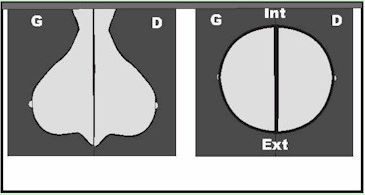
\includegraphics[scale=1.0]{images/mammogramMirror.png}
	\caption{A back to back position of the left and right breasts of both the MLO and CC views, Mammo}
  	\label{fig:mammogramMirror}
\end{figure}

	Masses are three-dimensional lesions in the sense that they're seen on multiple views. The location of a mass may be determined through the analysis of multiple views where observable masses are suspicious of malignancy. Size does not determine the malignancy of a mass, except if on successive views, the size of the mass regularly increases. Masses can be distinguished in five different types presented in figure \ref{fig:mammogramMassTypes}: round, oval, lobular, irregular, and architectural distortion  \cite{mammogramMass}.

\begin{figure}[h]
	\centering
  	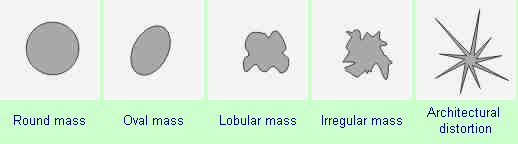
\includegraphics[scale=0.8]{images/mammogramMassTypes.png}
	 \caption{The five different types of mammogram masses, Mammo}
  	\label{fig:mammogramMassTypes}
\end{figure}

	Mass margins must also be detailed during analysis specifically the ROI they cover. As such, the five different margin types include circumscribed (well-defined and sharply demarcated), microlobulated (small circled line the edges), obscured, indistinct or ill-defined, and spiculated as seen in figure \ref{fig:mammogramMargin}. The obscured margins are due to adjacent normal tissue overlapping. Indistinct or spiculated margins illustrate the invasion of the malignant tumour into surrounding healthy tissue \cite{mammogramMass}.

\begin{figure}[h]
	\centering
  	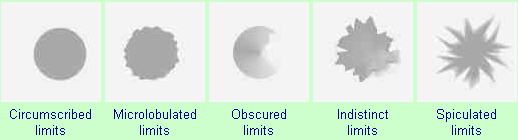
\includegraphics[scale=0.8]{images/mammogramMargin.png}
	 \caption{The five different types of mammogram mass margins, Mammo}
  	\label{fig:mammogramMargin}
\end{figure}

	 Generally, round, oval, or lobulated masses with circumscribed limits are benign tumors with only little known cases not following this rule \cite{regularBreastMasses}. Round masses with obscured limits are difficult to analyze often mimicking a cancer mass with ill-defined borders. In light of this, further breast examinations are performed. Masses with lobulated or microlobulated limits are suspicious of malignancy where the more lobulated the limits are, the greater the risk of malignancy. Masses with indistinct limits are also suspicious of malignancy \cite{irregularBreastMasses}. Masses observed as architectural distortions may also be a sign of malignancy, but they may also be a result of a surgical scar or unrelated diseases. Consequently, further breast examination must be performed. Masses with spiculated borders are highly suspicious of cancer as spicules illustrate invasion of the tumour into surrounding tissue \cite{irregularMasses}. \\

	Breast calcifications are small calcium deposits in women's breast tissue \cite{breastCalcification}. Calcification images should be detailed according to size, shape, number of calcifications, and distribution. Generally, larger calcifications (macrocalcifications) with regular or oval shapes are benign, while smaller, irregular calcifications (microcalcifications) are potentially malignant. Moreover, in analysing the size of calcifications, the sizes of microcalcification fall between 0.2 - 0.5 mm, while macrocalcification sizes are 2.0 mm or larger \cite{mammaryCalcifications}. \\

	When detailing the shape of calcifications, round, oval calcifications with uniform shape and size are suggestively benign, while irregular calcifications are potentially malignant. Furthermore, M. Le Gal proposed five types of microcalcifications according to shape with corresponding degrees of malignancy as detailed in figure \ref{fig:mammogramCalcificationTypes}: type I (tea-cup, annular, clear centres) with 0\% malignancy potential, type II (regularly punctiform) with 39\% malignancy potential, type III (dusty, salt particles) with 39\% malignancy potential, type IV (irregularly punctiform) with 59\% malignancy potential, and type V (vermicular punctiform) with 96\% malignancy potential \cite{mammaryCalcifications}.

\begin{figure}[h]
	\centering
  	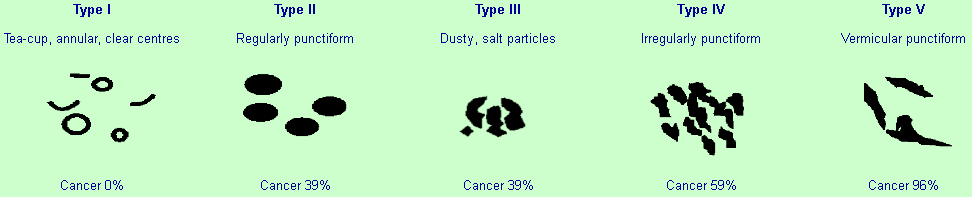
\includegraphics[scale=0.6]{images/mammogramCalcificationTypes.png}
	 \caption{The five different types of microcalcifications based on shape, Mammo}
  	\label{fig:mammogramCalcificationTypes}
\end{figure}

	Lastly, when analysing the number of calcifications, any number above four up to six microcalcifications is indicative of malignancy \cite{mammaryCalcifications}. \\

	After mammographic analysis and evaluation, the results are classified according to one of the following BI-RADS categories \cite{breastCancerScreeningAndDiagnosis}:

\begin{enumerate}
	\item{Category 0: Additonal imaging evaluation and/or comparison to prior mammograms is needed} \\
	The findings in the mammogram require additional imaging examination. Additional imaging examinations include ultrasound, MRI, special mammogram views, spot compression, and magnified views. Moreover, the mammogram of interest may be compared to past mammograms to identify changes over a period of time.

	\item{Category 1: Negative} \\
	The mammogram under study contain no significant abnormalities indicative of malignancy. The breasts appear healthy.

	\item{Category 2: Benign Findings} \\
	Like category 1, the mammogram of interest appear to contain no malignant abnormalities, but benign findings are present. Typical findings include benign-appearing macrocalcifications, oil cyst, or a lipoma.

	\item{Category 3: Probably Benign Findings; Short-Interval Follow-up Suggested} \\
	This is a mammogram that is usually benign, but further exploration should be performed to generate more stable readings.

	\item{Category 4: Suspicious Abnormality; Biopsy Should be Considered} \\
	The mammogram analyzed contains possible malignant abnormalities but not obviously malignant mammographically. A breast biopsy is recommended to verify malignancy.

	\item{Category 5: Highly Suggestive of Malignancy; Appropriate Action Should be Taken} \\
	The findings present in the mammogram are highly probable (> 95\%) of being malignant. Typical findings include spiculated mass or malignant-appearing microcalcifications. As such, breast biopsy is also recommended.

	\item{Category 6: Known Biopsy-Proven Malignancy; Appropriate Action Should be Taken} \\
	The findings on the mammogram have already been verified as malignant by a previous breast biopsy. This category is for mammograms that have cancer under study to see how well the cancer is responding to a particular treatment.
\end{enumerate}

\subsection{Machine Learning}

\qquad Machine learning is the science behind the ability of computers to act and learn concepts without being explicitly programmed, and improve learning over time through data and observations \cite{machineLearning}. To date, there are so many machine learning algorithms each with different uses for specific functions. Machine learning algorithms can be categorized into four types based on their purpose \cite{machineLearningTypes}:

\begin{enumerate}
	\item{Supervised Learning} \\
	In supervised learning problems, a data set is procured containing training examples or instances with associated correct labels or predictions. For example, the problem is to have the computer learn to classify handwritten digits. In a supervised learning approach, a data set must be acquired with thousands of pictures of handwritten digits along with labels identifying the correct number illustrated by image. The implemented algorithm would attempt to learn and acquire features from the images with respect to the number they represent in order to build a model to classify said images. The model would undergo several parameter tweakings and adjustments to achieve an optimal model. This process is referred to as training. Then, the model would be put to the test to classify handwritten digits on an unlabeled data set \cite{supervisedLearning}. Algorithms under supervised learning include Nearest Neighbor, Naive Bayes, Deision Trees, Linear Regression, Support Vector Machines (SVM), and Neural Networks.

	\item{Unsupervised Learning} \\
	In contrast to supervised learning, unsupervised learning involves training the computer with unlabeled data. This type of machine learning is typically used for pattern detection and descriptive modeling. Since there are no labels for which an algorithm can model relationships, unsupervised learning algorithms attempt to utilize techniques on the data to mine for rules, detect patterns, and summarize and group the data. Some common algorithms include k-means clustering and Association Rules.

	\item{Semi-supervised Learning} \\
	Semi-supervised learning involves a combination of the first two types. In order for supervised learning to be at its most effective, a large labeled data set is required. However, in practical situations, the cost of labeling is high, and, in some fields, a large fully-labeled data set lacks. So, in the absence of correct labels in the majority of the observations but present in few, semi-supervised learning algorithms may be implemented.
\end{enumerate}

	Furthermore, there are algorithms centered on a specific technique of machine learning called deep learning (DL). The main advantage of DL algorithms over ML algorithms is that DL algorithms can generate new features from existing ones in the training data set, while in ML algorithms, the features must be accurately identified which can be costly. Therefore, DL algorithms save more time when dealing with large, big complex data \cite{advantageDeepLearning}. \\

	Artificial neural networks (ANN), inspired by the biological structure of the human brain, are machine learning algorithms applied on the computer to perform specific tasks such as clustering, classification, pattern recognition, etc. A typical ANN contains hundreds of interconnected single units, artificial neurons, connected with coefficients (weights), which constitute the neural structure and are grouped and separated in layers. The behavior of an ANN depends on several factors such as the activation function of a neuron, the weights of each neuron, biases of each layer, the learning rule of the ANN, the architecture itself, etc. The output of a single neuron is determined by the weighted sum of the inputs passed through the activation function \cite{artificialNeuralNetworks}. \\

	During training, the training set is passed through the network, and the output obtained is compared with the actual value. The difference between the predicted output and the actual value is referred to as the error. The objective of training the network is to achieve a model where the parameters are optimized in such a way that the error in predictions is minimized specifically the error converges to a local minimum \cite{artificialNeuralNetworks}. \\

\subsection{Convolutional Neural Networks}
\qquad Convolutional Neural Network (CNN) is a common DL algorithm and a special case of ANNs. Historically, CNNs are mainly used for image recognition tasks specifically object detection and classification, due to their ability to learn higher-order features. A CNN is primarily composed of one or more convoluational and pooling (or subsampling) layers and then followed by one or more fully-connected layers. Figure \ref{fig:CNN} illustrates how a standard CNN architecture handles a vehicle image classification task. An image is input into the network where it undergoes several stages of convolution and pooling. The features extracted from the process are fed into the fully-connected neural network. Finally, the last fully-connected neural network outputs the predicted classification \cite{convolutionalNeuralNetworks}.

\begin{figure}[h]
	\centering
  	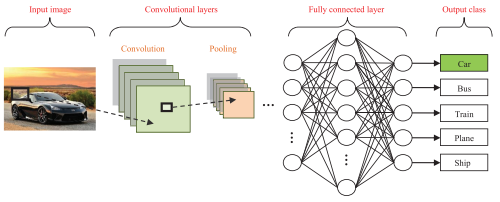
\includegraphics[scale=1.0]{images/CNN.png}
	 \caption{An intuitive overview of a standard CNN, Mammo}
  	\label{fig:CNN}
\end{figure}

	In the convolutional layer, features are extracted, and the feature representations of the input image is obtained. The convolutional layer's parameters involves a set of learnable filters typically small in dimension but extends through the full depth of the input volume (i.e. a filter for the first layer of size 5x5x3, with 5x5 height and witdth, and depth 3 for color channels). In the processing of the input volume, the filter slides (convolves) across the width and height of the input volume, while dot products are computed from the filter entries and the input. Typically, the first convolutional layers learn low-level features like edges or blotches of some color, while the latter layers learn higher level features \cite{convolutionalLayers}. Figure \ref{fig:convolutionalLayer} illustrates how convolution works. \\

\begin{figure}[h]
	\centering
  	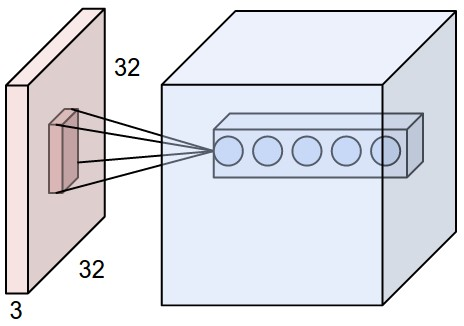
\includegraphics[scale=0.5]{images/convolutionalLayer.jpeg}
	 \caption{An illustration of an input volume (i.e. 32x32x3 input image) at the left and the first convolutional layer (a volume of neurons) to the right; image, Mammo}
  	\label{fig:convolutionalLayer}
\end{figure}

	The pooling layer, commonly placed in succession with several convolutional layers, serves to progressively reduce the spatial size of the representation in order to reduce the amount of parameters and computational costs in the network. There are two types of pooling namely average pooling and max pooling. Figure \ref{fig:poolingLayer} illustrates the difference between the two types \cite{convolutionalNeuralNetworks}. \\

\begin{figure}[h]
	\centering
  	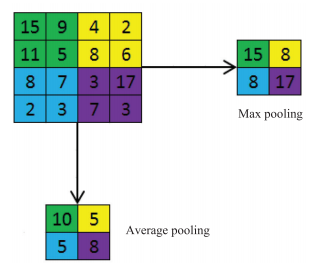
\includegraphics[scale=0.8]{images/poolingLayer.png}
	 \caption{Average pooling vs max pooling, Mammo}
  	\label{fig:poolingLayer}
\end{figure}

	In figure \ref{fig:poolingLayer}, a common pooling layer form is used where the filter size is 2x2 applied with a stride of 2. The input image here has a size of 4x4. After pooling is applied, max pooling outputs the maximum value of each 2x2 region, while average pooling outputs the average of each region. \\

	Lastly, the fully-connected layers interpret the feature representations extracted from the convolutional and pooling layers in order to arrive at a conclusion. The last layer here outputs the predicted class label.

\subsection{Residual Neural Networks}
\qquad According to He et. al \cite{Resnet}, the motivation behind Residual Neural Networks (ResNet) is a property of CNNs: as more layers are stacked (as the CNN goes deeper), the levels of features integrated by the network are enriched which would entail better model generalization. However, as a CNN goes deeper, the network becomes more difficult to train due to the problem of vanishing and exploding gradients. Moreover, when deeper networks are able to start converging, a degradation problem occurs where, due to the increase in network depth, the accuracy becomes saturated and then degrades rapidly resulting to higher training error. \\

	In their study \cite{Resnet}, the authors attempt to address the degradation problem by introducing a deep residual learning framework. In their network, instead of having some stacked layers fit a desired underlying mapping, they let the stacked layers fit a residual mapping. The authors have hypothesized that it is easier to optimize the residual mapping than to optimize the underlying, original mapping. The construction of such residual mapping can be realized by CNNs with "shortcut connections." Shortcut connections are those skipping one or more layers through the use of identity mapping, where the outputs are added to the outputs of the stacked layers as seen in figure \ref{fig:resNetSample}. \\

\begin{figure}[h]
	\centering
  	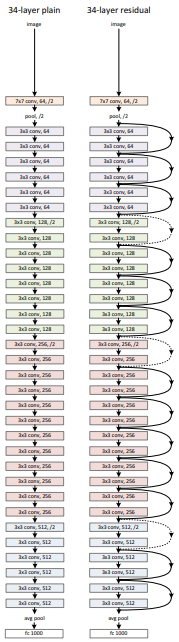
\includegraphics[scale=0.8]{images/resnet.png}
	 \caption{Left: a plain CNN with 34 parameter layers. Right: a RNN with 34 parameter layers. The dotted shortcuts increase dimensions, Mammo}.
  	\label{fig:resNetSample}
\end{figure}

	The authors have provided comprehensive evidence that their proposed residual learning framework is effective as they've obtained excellent results on the ImageNet classification data set with their 152-layer RNN where they obtained a 3.57\% top-5 error, and won 1st place in the ILSVRC 2015. \\

	As stated, the network architecture used is a pretrained ResNet-50 which is a ResNet with 50 parameter layers.
\clearpage